%------------------------------début entêtes-----------------------------------------
\pagestyle{fancy}

\renewcommand{\footrulewidth}{1pt}

\fancyhead[L]{État de l'art}
\fancyhead[C]{\thepage}
\fancyhead[R]{Information de base}

\fancyfoot[L]{Ny Hoavy Nomena}
\fancyfoot[C]{\thepage}
\fancyfoot[R]{Annotation automatique d'images}

%------------------------------fin entêtes-------------------------------------------

%\chapter{Généralités et applications de l'apprentissage profond} \label{genetap}
\chapter{Etat de l'art de l'apprentissage profond} \label{genetap}
Ce chapitre présente l'apprentissage profond. L'information de base, que nous avons jugée utile pour la compréhension de ce rapport, se porte sur:
\begin{itemize}
\item l'apprentissage profond en général dans la première section
\item suivi de ses applications dans le cadre des recherches en annotation automatique d'images dans la seconde section, à savoir: la vision par ordinateur, le traitement automatique de texte et la mise en correspondance des caractéristiques visuelles et textuelles.
\end{itemize}

\smallskip

\section{Généralités} \label{generalite}

\subsection{Apprentissage automatique et apprentissage profond}
L'apprentissage profond, \textit{"deep learning"}, est une méthode d'apprentissage automatique \textit{"machine learning"} basée sur les réseaux de neurones artificiels. L'apprentissage par expérience permet à l'ordinateur d'acquérir des connaissances dont il a besoin pour effectuer une tâche précise à partir de \textbf{données issues de phénomènes réels} sans l'intervention d'un opérateur humain.\\
\smallskip
Mitchell \cite{mitchell1997machine} : \textit{“A computer program is said to learn from experience E with respect to some class of tasks T and performance measure P , if its performance at tasks in T , as measured by P, improves with experience E.”}
\smallskip \\
Pour une tâche donnée, un algorithme d'apprentissage permet à un modèle d'acquérir une expérience. Cette expérience améliore sa performance pour effectuer cette tâche.\\
Dans le cas d'un apprentissage supervisé le modèle apprend par observation des exemples $x$ appartenant à  \{X\} associés à y appartenant à \{Y\}. L'algorithme d'apprentissage modélise une fonction $ f:X \mapsto Y$ par estimation de cette fonction. La fonction $f$ représente la relation entre les données d'entrée et de sortie et souvent représente la loi de probabilité conditionnelle de la distribution de $y$ sachant $x$ : $p(y|x)$.\\
Pour l'apprentissage non-supervisé, le modèle est mené à estimer la loi de probabilité $p(x)$ de la distribution  observée \{X\} par :
$p(x)= \prod_{i=1}^{n} p(x_{i}|x_{1},...,x_{i-1})$\\
\smallskip
\qquad L'apprentissage profond consiste surtout en l'apprentissage de l'ordinateur pour la compréhension d'un fait, par une représentation hiérarchique des concepts à partir de plusieurs couches. Cette représentation hiérarchique permet d'apprendre des concepts plus compliqués issus des relations entre les concepts les plus simples.

\subsection{Bref historique }
L'apprentissage profond a débuté dans les années 40. Il est l'aboutissement de l'évolution du domaine de Réseau de Neurones Artificiels (RNA)\cite{Goodfellow-et-al-2016-Book}.
\begin{itemize}
	\item \textbf{Cybernetics (1940 à 1960) :} a été le premier prédécesseur des modèles linéaires. Cette époque a été marquée par un modèle appelé \textit{"perceptron"} fabriqué par Rossenbatt en 1958 \cite{rosenblatt1958perceptron} qui a été inspiré par le travail de McCulloch et Pitts dans \cite{mcculloch1943logical} sur l'étude biologique de l'apprentissage. Grâce aux perceptrons ils ont pu implémenter un modèle capable de classifier une entrée dans 2 catégories (1 ou 0).

	\item \textbf{Connexionnisme (1980 à 1990) :} Depuis a émergé la science cognitive qui est un domaine pour l'étude de la pensée. Le connexionnisme est basé principalement sur le fait que l'interaction entre plusieurs neurones accroît l'intelligence. Une des grandes découvertes dans ce domaine est la rétropropagation \cite{hecht1989theory} qui est largement utilisée pour l'apprentissage des RNA.
	\item \textbf{Deep learning ou apprentissage profond (2006 à aujourd'hui) :} s'inspire de plusieurs domaines, pour améliorer les systèmes existants et créer des modèles profonds, spécialement les mathématiques appliquées : l'algèbre linéaire, la probabilité, la théorie de l'information et l'analyse numérique.\\
\end{itemize}
En 1998, Yan LeCun et al. ont déployé le premier système utilisant un modèle d'apprentissage profond LeNet-5 \cite{lecun1998gradient}. LeNet-5 a été modélisé pour la reconnaissance de l'écriture manuscrite (OCR) et intégré dans un système pour la reconnaissance de documents. Dans \cite{lecun1998gradient} Yan LeCun et al. décrivent LeNet-5 où ils évoquent une technique d'apprentissage nommé : GTN (Graph Transformer Networks). Ces derniers ont utilisé un réseau de neurones convolutif ou CNN (Convolutional Neural Network ou ConvNet) entraîné par un algorithme de descente de gradient : la rétropropagation. Ce modèle est aujourd'hui la base de la majorité des modèles d'apprentissage profond surtout appliqués à la vision par ordinateur.\\
Grâce aux larges données d'apprentissage, les chercheurs ont pu entraîner des modèles de réseau de neurones profond \footnote{la profondeur d'un réseau est définie par le nombre de couches formant le réseau d'où le nombre de paramètres}  en évitant le sur-apprentissage.\\
En 2012, Alex Krizhevsky et al.\cite{krizhevsky2012imagenet} ont remporté la première place lors d'un concours organisé par ImageNet : ImageNet ILSVRC en 2012 grâce à leur réseau de neurones convolutif profond: AlexNet. En résumé, AlexNet est composé de cinq couches de convolution et trois couches interconnectées utilisées comme classifieur. Pour ce modèle, on compte un total de 650.000 neurones et 60 millions de paramètres et il a servi à classifier 1,2 millions d'images suivants 1000 classes différentes issues de l'ImageNet ILSRVC-2010. Ce modèle a été entraîné dans un temps raisonnable (5 à 6 jours) en assignant  le traitement de calculs à des cartes graphiques programmables. 
%[2 GTX 580].
\\
Les grandes collections de données et les cartes graphiques programmables \footnote{GPUs : qui à la fois permettent les calculs en parallèle et atteignent les trillions de calculs par second}  ont rendu l'apprentissage profond plus accessible et ont contribué à l'accroissement des travaux dans ce domaine.
	
\smallskip


\subsection{Spécificité de l'apprentissage profond}
L'apprentissage automatique s'intéresse surtout aux problèmes et tâches qui sont subjectifs et qui ne peuvent pas être décrits précisément par un langage formel. Ces tâches sont trop complexes pour y appliquer des règles logiques et les programmer "en dur" [\textit{hard coding}]. Selon wikipédia  \cite{wikipediaapprentissage}, je cite: "La difficulté réside dans le fait que l'ensemble de tous les comportements possibles compte tenu de toutes les entrées possibles devient rapidement trop complexe à décrire (on parle d'explosion combinatoire) dans les langages de programmation disponibles. On confie donc à des programmes le soin d'ajuster un modèle permettant de simplifier cette complexité et de l'utiliser de manière opérationnelle." Comme exemple, on peut citer les problèmes de perception: reconnaissance d'objets et de formes ou vocales.\\
\qquad Un des avantages d'utiliser l'apprentissage profond par rapport aux autres algorithmes d'apprentissage est l'extraction des caractéristiques pertinentes des données pour résoudre le problème étudié. Cette étape est généralement effectuée lors d'un \textit{"feature engineering"} dans l'apprentissage automatique classique. En apprentissage profond, cette étape est assignée à l'algorithme lui même par  \textit{\textbf{"feature learning"}} (apprentissage de la représentation). Un autre problème rencontré lors d'un apprentissage automatique est l'identification des sources qui influencent les valeurs des données observées : \textbf{facteurs de variation}. Ces facteurs ne sont pas quantifiables et sont souvent difficiles à identifier. L'apprentissage profond introduit alors la représentation hiérarchique de l'entrée sur plusieurs couches du réseau. Les caractéristiques extraites des neurones d'une couche précédente sont alors pondérées et partagées pour former des caractéristiques plus complexes. Ainsi on peut facilement établir une représentation plus complexe à partir de la combinaison des caractéristiques issues des couches antérieures en augmentant la profondeur du réseau c'est-à-dire en ajoutant des couches supérieures.\\
\textbf{Le principal enjeu est d'agréger les variables et ses interactions dans les systèmes complexes en créant un modèle de basse dimension qui permet d'exliquer ces systèmes.}
L'apprentissage profond permet de généraliser les problèmes. Grâce à l'apprentissage hiérarchique des invariants qui sont caractéristiques du problème, ces modèles évoluent facilement en fonction des tâches auxquelles ils sont soumis.\\
\smallskip
\section{Application dans le cadre de nos recherches} \label{application}
Un algorithme d'apprentissage profond a pour objectif de créer un modèle représentant une fonction ou système complexe 
%dans un espace de plus basse dimension (réduite) 
pour avoir une meilleure représentation des données les plus complexes grâce à un réseau de neurones artificiels (RNA).\\
\smallskip
\qquad Les réseaux de neurones artificiels ont la capacité de modéliser une fonction $f$ linéaire ou non-linéaire. La combinaison de couches linéaires qui effectuent des translations sur leurs entrées et des couches non-linéaires définies par la fonction d'activation non-linéaire de chaque neurone (ex : ReLu, Tanh) permet d'approximer toute fonction  \footnote{Borel mesurable, toute fonction de projection d'une espace discrète de dimension finie à une autre. (voir la théorie de l'approximation universel cité dans \cite{baldi1989neural})}. \\
En général, un réseau de neurones profond est défini par une succession de plusieurs couches faisant intervenir plus de paramètres qui nous autorise à approximer les fonctions les plus complexes.
Les informations générales concernant les réseaux de neurones artificiels et leur apprentissage sont détaillées dans\textbf{ l'Annexe}.\\
\qquad Les sections suivantes présentent les travaux étudiés dans le domaine de l'apprentissage profond. Ces travaux concernent l'application de l’apprentissage profond dans le domaine de la vision par ordinateur (\ref{vo}), le traitement automatique du langage naturel (\ref{taln}) et l'appariement des images et textes (\ref{associationit}).\\

\subsection{Application dans le domaine de la vision par ordinateur} \label{vo}

L'utilisation de l'apprentissage profond dans le domaine de la vision par ordinateur est la reconnaissance d'objets et de formes à partir des réseaux de neurones convolutifs ou Convolutional Neural Network (CNN) en anglais.\\
\smallskip

La reconnaissance a pour objectif de développer un algorithme qui soit capable de recevoir en entrée une image et de faire sortir la classe des objets (dans l'image) si on parle de catégorie d'objets et la référence d'un objet précis si on parle d'instance d'objets.
La difficulté de la reconnaissance visuelle par un ordinateur réside sur la variation extrême de la forme et de l'apparence des objets d'une classe (par exemple un ordinateur) dans le monde réel. En effet, si l'apparence n'était pas aussi variable, il suffirait d'effectuer une correspondance exhaustive à une base de données, ce qui n'est pas le cas.	\\
\smallskip
Un réseau de neurones convolutifs est une succession de couches de neurones appliquant à chaque entrée l'opérateur convolution pour exploiter la structure spatiale des données en entrée (par exemple une matrice de pixels pour les images). La convolution permet d'extraire les caractéristiques d'une image numérique en appliquant un filtre, \textit{convolution kernel}, suivant les axes possibles: hauteur, largeur et la profondeur (les canaux rouge, bleu et vert) de cette image. Une couche de convolution utilise la convolution discrète pour une transformation linéaire des valeurs des pixels en préservant l'ordre de ces valeurs \footnote{chaque pixel étant fortement corrélé avec les pixels voisins} dans l'espace local de l'image . Le filtre varie en fonction des effets désirés. La figure \ref{detectcont} illustre une détection de contours sur l'image en entrée par convolution.
Les réseaux de neurones convolutifs adoptent des principes importants pour la représentation des entrées: la connectivité locale et le partage des paramètres.

La connexion locale des neurones des couches adjacentes assure que les filtres appris produisent des caractéristiques locales les plus fortes à un motif  localisé. Précisément, chaque neurone n'est connecté qu'à une sous-région (champ réceptif local) correspondant à un certain nombre de neurones voisins dans la couche précédente.

Le partage des paramètres utilisés par l'opération de convolution signifie que, plutôt que d'apprendre un ensemble distinct de paramètres pour chaque emplacement, le modèle apprend un seul ensemble. Ainsi tous les neurones dans une couche de convolution donnée détectent exactement la même caractéristique. 
\medskip
\begin{figure}[h]
	\begin{center}
	 	
		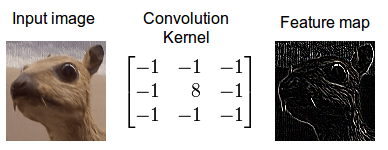
\includegraphics[width=0.7\textwidth]{convolution} 
		\caption{Détection de contours par convolution discrète. Source: \cite{wikipedia} \label{detectcont}}
	\end{center}

\end{figure}

Ce type de modèle est utilisé pour la classification d'images  car il fournit une bonne représentation de l'image par représentation hiérarchique issue des différentes couches de convolution et des couches de mise en commun (\textbf{pooling}) consécutifs. Cette architecture permet de réduire la sensibilité en translation, rotation et échelle ou aux faibles déformations de la représentation apprise.\\
%représentation et capture des invariants ou symétrie
	\smallskip
Dans les paragraphes suivants nous décrivons la structure des modèles utilisés pour la classification d'images que nous avions étudiées dans nos travaux.

\smallskip

\subsubsection{AlexNet \cite{krizhevsky2012imagenet}}
Ce modèle a été établi par Alex Krizheski et al. Le modèle est composé de 9 couches successives (voir tableau \ref{tab:alexnet}) dont cinq sont des couches de convolution pour l'extraction des caractéristiques de l'image et trois sont des couches entièrement connectées pour la classification de cette image.\\
\begin{table}
	\caption{\label{tab:alexnet} Tableau récapitulatif de l'architecture Alexnet \cite{krizhevsky2012imagenet} }
	\begin{tabular}{|M{6cm}|M{4cm}|M{6cm}|}
 		\hline
 		 Couche & Entrée & Filtres (nombre – dimensions – pas) ou Nombres de sortie\tabularnewline
 		\hline
 		 Première & Image de 224$\times$224$\times$3 & 96-11$\times$11$\times$3-4 \tabularnewline
 		Seconde & Sortie 1-ère couche + Normalisation et pooling & 256 - 5$\times$5$\times$48 \tabularnewline \hline
		 Troisième & Sortie 2-nde couche + Normalisation et pooling & 384 - 3$\times$3$\times$256 \tabularnewline \hline
 		Quatrième & Sortie 3-ème couche & 384 - 3$\times$3$\times$192 \tabularnewline \hline
  		Cinquième & Sortie 4-ème couche & 256 - 3$\times$3$\times$192 \tabularnewline \hline
 		 3 couches interconnectées: FC6 - FC7 - FC8 & Sortie 5-ème couche + 		Normalization et pooling & 4096 \tabularnewline \hline
		Une couche de sortie pour les 1000 classes & Sortie fully connected layer + Softmax & 1000 \tabularnewline
		\hline
\end{tabular}
\end{table}

AlexNet utilise deux techniques pour l'accélération de l'apprentissage par rétropropagation et éviter le sur-apprentissage : ReLu ou Rectified Linear Unit comme fonction d'activation des neurones et Local Response Normalization pour la normalisation.


\smallskip

\subsubsection{VGG - OxfordNet \cite{simonyan2014very}}
VGG ou OxfordNet sont des modèles créés par un groupe de l'université d'Oxford : Visual Geometry Group. Le groupe ont déployé ses deux meilleurs modèles: VGG-16 (16 couches) et VGG-19 (19 couches). \\
%La séquence de filtre 3$\times$3 permet d'extraire des caractéristiques plus complexes au lieu d'utiliser des larges convolutions comme 5$\times$5 et 7$\times$7 (voir bloc 3, 4,5 du modèle E) réduisant le nombre de paramètres mise en jeu pour des résultats sensiblement similaires.\\
\smallskip

\subsubsection{GoogLeNet \cite{szegedy2015going} et Inception}
Christian Szegedy et al. dans \cite{szegedy2015going} ont présenté une autre architecture nommée GoogleNet. Leur contribution a été de créer un modèle plus profond (22 couches) pour améliorer les performances des réseaux profonds tout en réduisant le coût du traitement. Le module "inception" a été alors créé qui est une combinaison de convolutions (de filtre 1$\times$1, 3$\times$3 et 5$\times$5) et de pooling en parallèle.

 L'inception a été amélioré par Christian et Serguei présenté dans \cite{ioffe2015batch} et \cite{szegedy2015rethinking}. La première amélioration \cite{ioffe2015batch} a été la normalisation des données pour chaque lot : batch-nomalized inception ou inception V2. La normalisation consiste à centrer et réduire les entrées pour chaque couche. L'architecture de la seconde amélioration inception V3 \cite{szegedy2015rethinking}  est présentée dans le tableau \ref{tab:inceptionv3}. 
 %\textbf{Les améliorations se résument à une factorisation des convolutions utilisées dans le réseau (comme l'utilisation des convolutions de filtre 3$\times$3 similaire à VGGNet) et à une balancement de la largeur (nombre de filtres par étape) et la profondeur du réseau pour optimiser sa performance.}

\begin{table}
	\caption{\label{tab:inceptionv3} Tableau récapitulatif de l'architecture Inception V3 \cite{krizhevsky2012imagenet} }
	\begin{tabular}{|M{6cm}|M{6cm}|}
 		\hline
 		Type & Taille entrées \tabularnewline \hline
 		Convolution & 299$\times$299$\times$3 \tabularnewline \hline
 		Convolution & 149$\times$149$\times$32 \tabularnewline \hline
 		Convolution padded & 147$\times$147$\times$32 \tabularnewline \hline
 		Pooling & 147$\times$147$\times$64 \tabularnewline \hline
 		Convolution & 73$\times$73$\times$64 \tabularnewline \hline
 		Convolution & 71$\times$71$\times$80 \tabularnewline \hline
 		Convolution & 35$\times$35$\times$192 \tabularnewline \hline
 		3 $\times$ inception & 35$\times$35$\times$288 \tabularnewline \hline
 		5 $\times$ inception & 17$\times$17$\times$768 \tabularnewline \hline
 		2 $\times$ inception & 8$\times$8$\times$1280 \tabularnewline \hline
 		Pooling & 8$\times$8$\times$2048 \tabularnewline \hline
 		Linear & 1$\times$1$\times$2048 \tabularnewline \hline
 		softmax & 1$\times$1$\times$1000 \tabularnewline
		\hline
\end{tabular}
\end{table}
\medskip
Ces modèles ont été entraînés pour classifier des millions d'images de la collection ILSVRC ou ImageNet Large Scale Visual Recognition Challenge \cite{russakovsky2015imagenet} sur 1000 classes différentes.\\
Ces modèles pré-entrainés peuvent être utilisés pour effectuer des tâches suffisamment similaires (par exemple classification d'autres classes que les classes d'ILSRVC \cite{liuimage}) et accélèrent l’apprentissage du réseau par transfert des paramètres. Pour adapter ces modèles aux nouvelles tâches on procède alors à une \textit{fine-tuning }ou \emph{réglage fin} du modèle : classification de scènes \cite{szummer1998indoor} \cite{zhou2014learning}, détéction d'objets \cite{jitendramalikrich}, \cite{ren2015faster},\cite{wei2014cnn}. Ces modèles sont efficaces du fait qu'ils ont été entraînés sur un large ensemble de données de plusieurs classes pour détecter les caractéristiques et structures pertinentes des images.\\
Ces modèles sont aussi intéressants car, en tant que \textbf{descripteur}, ils permettent l'extraction des vecteurs caractéristiques des images ou  vecteurs descripteurs.  
 Des vecteurs caractéristiques peuvent être extraits à partir de ces modèles pour représenter les images en entrée et les utiliser dans d’autres applications plus complexes. \\

 
\smallskip
%\qquad Par exemple dans la figure suivante, les images sont représentés par les vecteurs descripteurs issus de la couche FC7 d'un modèle AlexNet (entraînés sur ILSRVC 2012) de dimension 4096 et projeter dans une espace à deux dimensions par l'algorithme t-SNE[35] [t-SNE permet une meilleure visualisation des données à grandes dimensions en préservant la distance entre les données]. On peut constater que les images ayant des caractéristiques visuelles similaires (couleurs, texture,..) et appartenant à la même classe (représente les même concepts et objets) sont voisins.

\subsection{Application sur le traitement automatique du langage naturel} \label{taln}
 Les problèmes étudiés dans le traitement automatique du langage naturel se concentrent sur une meilleure représentation des textes (mots, groupes de mots, phrases) pour apporter une connaissance à l'ordinateur sur leur signification et leurs propriétés en vue d'effectuer des tâches du TALN comme la recherche de mots clés, recherche de synonymes, la traduction,... . A la différence de certaines méthodes considérant chaque texte comme une combinaison possible des lettres de l'alphabet, les travaux suivants concernent une représentation par des vecteurs.  La représentation vectorielle facilite la résolution des problèmes d'analyse en utilisant les différentes propriétés et opérations vectorielles, comme le calcul de la distance vectorielle. \\

\subsubsection{Représentation vectorielle des mots}

 Une première représentation est la représentation par « sac-de-mots » bag of word en anglais. La représentation est basée sur la matrice de cooccurrence, qui est constituée par la fréquence des mots dans chaque document. La matrice est donc obtenue en comptant le nombre de fois où le mot apparaît dans chaque document. Chaque mot est alors représenté par  la ligne correspondante de la matrice de cooccurrence et le document par la colonne correspondante. Cette représentation en grande dimension ne capture que peu d'informations sur la signification de chaque mot.\\
\smallskip
D'autre part, la signification d'un mot est en référence avec les mots qui l'entourent. Les méthodes sont fondées par la constatation suivante : « Les mots qui apparaissent dans un même contexte ont tendance à avoir les mêmes significations » comme le formulait Harris \cite{harris1954distributional}. Ainsi Sahlgren M., \cite{sahlgren2008distributional} a proposé \textbf{« l'hypothèse de distribution »} pour quantifier la signification des mots en vue d'extraire leurs relations.\\
Les approches que nous avons étudiées concernent les méthodes de \textit{"word embedding"} utilisant les réseaux de neurones artificiels (RNA).\\
Les \textit{word embedding} sont des méthodes qui permettent de représenter les mots par des vecteurs à dimensions réduites (200-1000 mais largement inférieures à la taille du vocabulaire) en modélisant la relation entre les mots: sémantique et syntaxique. On définie le \textit{word embedding} par la projection des mots dans un espace vectoriel :\\
word-embedding: $W: mots \mapsto \mathbb{R}^{n}$\\
Pour les mots similaires (apparaissant dans le même contexte) $w_{s}$  $W(w_{s})$ sont plus proches (suivant la mesure de distance utilisée dans l'espace).\\
Cette représentation continue permet aussi de capturer des analogies entre les mots. Par exemple, les notions de genre et nombre en utilisant les opérateurs arithmétiques vectoriels :\\
$\begin{matrix}
W('woman')- W('man') &\simeq  W('aunt')- W('uncle') \\
 & \simeq W('queen') - W('king')
\end{matrix}
$


 Pour cette représentation distributive des mots à partir des RNA, Mikolov et al.  \cite{mikolov2013efficient} ont proposés deux 2 modèles n-gramme appelés "modèles word2vec" : skip-gram et cbow (continuous bag of words). Skip-gram et cbow sont 2 architectures de RNA simples composés de 3 couches illustrés par le figure \ref{fig:wor2vec}  :\\
\medskip
\begin{figure}[h]
\label{fig:wor2vec}
	\begin{center}
		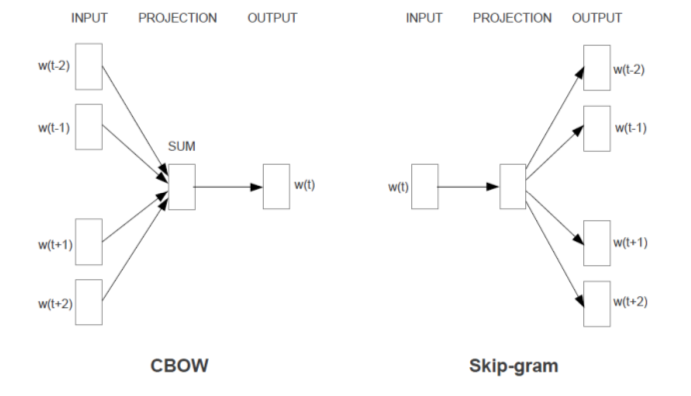
\includegraphics[width=0.7\textwidth]{word2vec}
		\caption{Architecture des modèles cbow et skip-gram de Word2Vec \cite{mikolov2013efficient}}
	\end{center}
\end{figure}


En général, les modèles word2vec sont entraînés pour prédire les mots voisins et obtenir une meilleure représentation des mots.
Ces architectures construisent des fenêtres de contexte obtenues en prenant les c mots qui précédent et les c mots qui suivent un mot appelé \textbf{mot central}. Le modèle skip-gramm est entrainé pour prédire les mots de la fenêtre de contexte pour un mot central donné. Tandis que cbow est entraîné pour l'inverse. Pour cela, skip-gram prend en entrée un mot central et pour le modèle cbow un sac-de-mots (les mots du contexte). La projection de ces entrées par une matrice globale (partagée par les mots) est capturée par la couche cachée. Pour le modèle skip-gramm, le mot central représenté en sac-de-mot binaire est projeté dans la couche cachée par la matrice de \textit{word embedding}\label{text:wordembed}. Ensuite les mots du contexte, chacun représenté en sac-de-mot binaire, sont projetés dans la couche cachée par la matrice de \textit{contexte embedding}. En sortie, on calcule le produit scalaire de la projection du mot central et chaque projection des mots du contexte  pour obtenir le score de similarité. La fonction softmax permet de normaliser la sortie en probabilité.\\

La méthode par descente du gradient est utilisée pour entraîner les modèles à trouver les matrices de projection: word embedding et contexte embedding qui maximisent la probabilité de la similarité entre le mot central et les mots du contexte. Concrètement, le modèle est entraîné en maximisant les fonctions log-vraisemblance (dans tout le vocabulaire) données par les formules suivantes:
\begin{eqnarray}  \frac{1}{T} \sum_{t=1}^{T} \log  p(w_{t}|w_{t-\frac{c}{2}}...w_{t+\frac{c}{2}}) \end{eqnarray} pour le modèle cbow 
\begin{eqnarray} \frac{1}{T} \sum_{t=1}^{T}  \sum_{j= t-c, j\neq t}^{t+c} \log  p(w_{j}|w_{t})\end{eqnarray} pour le modèle skip-gram\\
$T$ : taille des données d'apprentissage\\
$c$ : taille maximum de la fenêtre de contexte\\
%L'apprentissage est effectué par approximation des erreurs par la méthode de "échantillons négatifs" ou \textit{ "negative sampling" } introduite par Mikolov et al dans \cite{mikolov2013distributed}\\

\subsubsection{Modèles neuronaux pour la génération de phrases} \label{phrasegen}

 Dans cette partie une phrase est traitée en tant que séquence de mots ordonnés. %et dont la signification d'un mot dépend de sa position dans cette séquence.
La génération d'une phrase est plus complexe car elle est déterminée par les représentations des expressions (mots) qui les constituent et les règles de grammaire utilisées pour les combinés. 

Les modèles de langue neuronaux sont utilisés pour prédire une séquence de mots dans les systèmes de reconnaissance vocale, la traduction automatique et les systèmes questions-réponses. Ces modèles sont entraînés pour estimer la loi de probabilité de la séquence de m mots $p(w_{1},…,w_{m})$ par apprentissage des réseaux de neurones.\\
Dans les modèles n-grams, cette probabilité  est conditionnée par une fenêtre des n mots (n fixe).
\begin{eqnarray}
p(w_1,...,w_m) = \prod_{t=1}^{m} p(w_t | w_{1},...,w_{t-1}) \approx \prod_{t=1}^{m} p(w_t | w_{t-(n-1)},...,w_{t-1})
\end{eqnarray}
$w_{t-(n-1)},...,w_{t-1}$ : représente le contexte.\\
Ces modèles sont limités à la représentation de séquences car ils sont conditionnés par la fréquence des coocurences des n-grammes dans le document. Il est rare que des n-grammes (pour n assez grand) correspondent exactement dans des phrases similaires vu \textit{l'infinité} des variations possibles. 
Ainsi, les réseaux de neurones récurrents ont été introduits \cite{mikolov2010recurrent} \cite{mikolov2011extensions}.
L'avantage d'utiliser les réseaux de neurones récurrents, par rapport aux réseaux de neurones simples, est leur capacité à capturer une meilleure  représentation des séquences de données de tailles variables \cite{schmidhuber2015deep}.\\
Grâce à la représentation de l'historique des mots à partir de la couche cachée, les réseaux de neurones récurrents permettent de modéliser cette probabilité en prenant en compte tous les mots précédents (de nombre variable) sous forme de contexte. \\
%Les réseaux de neurones récurrents utilisent les couches cachées pour représenter tous les mots qui précédent un mot à une position donnée en reprenant l'état caché précédent pour calculer l'état caché présent.
%etat caché: allant de xt à xt+1

A un instant $t$, les paramètres des réseaux de neurones récurrents sont définis par :
\begin{eqnarray}
h_{t} = \sigma(W^{(hh)} h_{t-1} + W^{(hx)} x_{t})\\
\hat{y_{t}} = softmax(W^{(S)} h_{t})
\end{eqnarray}\\
$ x_{t} \in \mathbb{R}^{d}$ est le vecteur (sac-de-mot binaire) qui représente le mot courant à l'instant t\\
$h_{t}$ : est la sortie de la couche cachée\\
	$W^{(hh)} \in \mathbb{R}^{D_{h}\times D_{h}}$ sont les paramètres qui conditionnent la sortie de la couche cachée à l'instant précédent $t-1$\\
	$W^{(hx)}\in \mathbb{R}^{D_{h}\times d}$  est la matrice de projection de l'entrée. Elle correspond à la matrice de \textit{word embedding} citée en \ref{text:wordembed}.\\
%sont les paramètres qui conditionnent l'entrée $x_{t}$\\
	$\sigma$ est une fonction non-linéaire (par exemple sigmoid)\\
$\hat{y_{t}} \in \mathbb{R}^{|V|}$ permet de générer le mot suivant de la séquence observée sachant le contexte (à partir de $h_{t-1}$) et le mot observé (représenté par $x_{t}$), ceci en générant la probabilité pour chaque mot du vocabulaire à l'instant $t$ :$ \hat{p}(x_{t+1}=v_{j}|x_{t},...,x_{1})= \hat{y}_{tj}$\\
	$W^{(S)} \in \mathbb{R}^{|V| \times D_{h}}$\\
$|V|$ est la taille du vocabulaire\\
Le réseau est entraîné par la maximisation de vraisemblance en minimisant la fonction de l'entropie croisée à l'instant $t$ (sommée sur tout le vocabulaire)[equation \ref{eq:jt}]  par  \textbf{rétropropagation à travers le temps} \cite{werbos1990backpropagation}.
\begin{eqnarray}
\label{eq:jt}
J^{(t)}(\theta) = -\sum_{j=1}^{\left | V \right |}y_{tj}\times \log(\hat{y}_{tj})
\end{eqnarray}



\begin{figure}[h]
	\begin{center}
		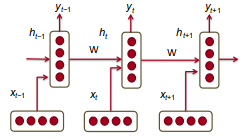
\includegraphics[width=0.4\textwidth]{rnn}
		\caption{Représentation du réseau de neurones récurrents }
	\end{center}
\end{figure}
\smallskip
Le but d'un réseau neuronal récurrent est de propager le contexte  étape par étape, cependant cette technique présente des défauts sur des séquences assez longues. Le problème se rapporte à la disparition (ou explosion) du gradient lors de la rétropropagation qui compromet la performance de ces modèles \cite{hochreiter1998vanishing}. \\
De nouveaux types de réseaux de neurones récurrents plus performants ont émergé pour contourner  le problème de la disparition du gradient à savoir : les GRU : \textit{Gated Reccurents Units} et LSTM : \textit{Long-Short-Term-Memories} \cite{hochreiter1997long}. Ces derniers sont des extensions des réseaux de neurones récurrents simples en utilisant des unités d'activation plus complexes. Ils sont conçus de manière à avoir une mémoire plus persistante pour faciliter la capture des dépendances à long terme. Dans tout ce qui suit, la représentation de ces réseaux récurrents est tirée de http://cs224d.stanford.edu qui est plus élaborée et plus compréhensible.\\

Le modèle GRU est composé des unités (\textit{gates}) suivants :\\
$\begin{matrix}
z_{t}=\sigma(W^{(z)}x_{t}+ U^{(z)}h_{t-1}) & update\, gate\\ 
r_{t}=\sigma(W^{(r)}x_{t}+ U^{(r)}h_{t-1}) & reset\, gate\\ 
\check{h}_{t} = \tanh(r_{t} \circ Uh_{t-1}+Wx_{t}) & New memory\\ 
h_{t}=(1-z_{t}) \circ \check{h}_{t} + z_{t} \circ h_{t-1}& hiden state 
\end{matrix}
$
\\
%Génération d'une nouvelle mémoire: $\check{h}_{t}$  est une nouvelle unité  utilisée pour synthétiser le mot en entrée (représentée par $x_{t}$) dans le contexte  de la séquence observée (à partir de l'état caché $h_{t}$)\\
%Reset Gate : $ r_{t}$ est la pondération de l'état caché $ h_{t-1}$ pour la synthétisation $\check{h}_{t}$.\\
%Update Gate :  $ h_{t-1}$ est pondéré par $z_{t}$ lors de la propagation de l'état suivant.\\
%		Si $z_{t} \approx 1$ $ h_{t-1}$ est recopié sur $h_t$.\\
%\qquad		Si $z_{t}\approx 0$ $\check{h}_{t}$ est propagé vers l'état caché \\
%Hiden State : $h_{t}$ est généré en utilisant l'état caché précédent $ h_{t-1}$ et la nouvelle mémoire générée $\check{h}_{t}$ en prenant compte de l'update gate $z_{t}$.\\
%$\sigma$ est la fonction d'activation de l'unité (souvent la fonction sigmoïde)\\
%\smallskip
%Les modèles GRU sont entraînés par rétropropagation du gradient temporelle sur les paramètres : $W$ et $U$.\\

%\begin{figure}[h]
%	\begin{center}
%		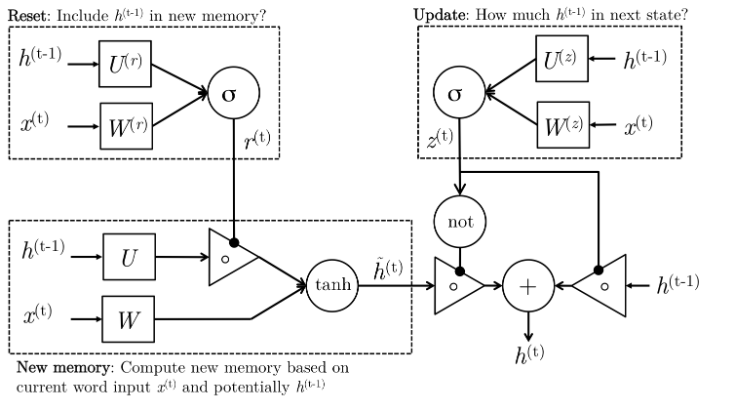
\includegraphics[width=0.5\textwidth]{gru}
%		\caption{Illustration du modèle GRU http://cs224d.stanford.edu}
%	\end{center}
%\end{figure}
%\smallskip

%L'architecture du LSTM est illustrée par la figure [figure LSTM]\\
 Mathématiquement, les unités d'un LSTM est définie par :\\

$\begin{matrix}
i_{t}=\sigma(W^{(i)}x_{t}+ U^{(i)}h_{t-1}) & input\, gate\\ 
f_{t}=\sigma(W^{(f)}x_{t}+ U^{(f)}h_{t-1}) & forget\, gate\\
o_{t}=\sigma(W^{(o)}x_{t}+ U^{(o)}h_{t-1}) & output\, gate\\ 
\check{c}_{t} = \tanh(W^{(c)}x_{t}+ U^{(c)}h_{t-1}) & new\, memory\, cell\\
c_{t}=f_{t} \circ c_{t-1}+i_{t} \circ \check{c}_{t} & final\, memory\, cell\\
h_{t}=o_{t} \circ \tanh(c_{t})& hiden state 
\end{matrix}$

%$\check{c}_{t}$ est la nouvelle mémoire générée à partir du mot en entrée.\\ $x_{t}$ et l'état caché $ h_{t-1}$. \\
%$i_{t}$ input gate et $f_{t}$ forget gate . \\
%%peuvent être interprétés comme interrupteur pour inciter le modèle à considérer le mot en entrée ou à oublier la mémoire précédente	
%$o_{t}$ pour output gate pondère la mémoire qui sera propagée.

%\begin{figure}[h]
%	\begin{center}
%		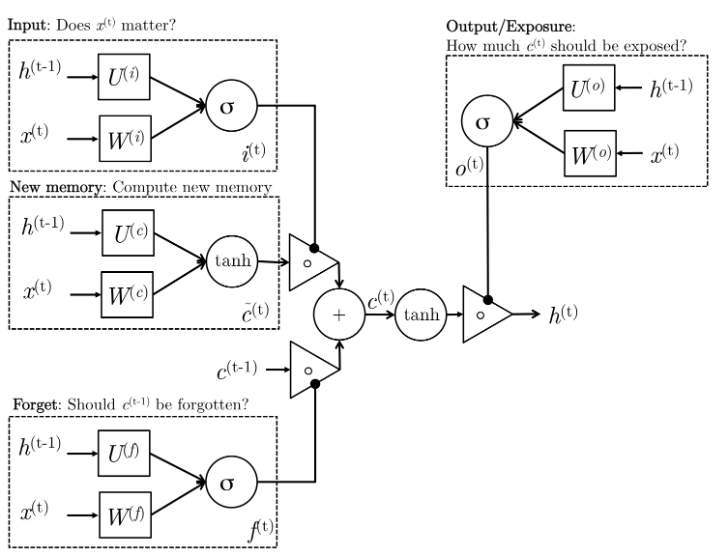
\includegraphics[width=0.4\textwidth]{lstm}
%		\caption{Illustration du modèle LSTM http://cs224d.stanford.edu}
%	\end{center}
%\end{figure}
%\smallskip
 Avec ses unités, un LSTM est capable d'apprendre des séquences d'informations assez longues et complexes.\\

 Ces modèles de langue neuronaux sont utilisés dans le TALN: les systèmes de traduction, la reconnaissance automatique de la parole et à la description des images \cite{mao2015learning} \cite{mikolov2010recurrent}, \cite{mikolov2011extensions},\cite{mikolov2013distributed} \cite{graves2014towards} \cite{sutskever2014sequence}


\smallskip
